\documentclass[../main.tex]{subfiles}

\begin{document}
TO BE COMPLTED

\subsection{CTF Correction}
When comparing experimental images to reference ones, the \gls{ctf} must be taken into consideration. Most implementations choose to apply the \gls{ctf} to the reference images. The main drawback of this election is that the \gls{ctf} varies across images, hence, the \gls{ctf} needs to be re-applied to the reference gallery for each experimental image\cite{scheres2005}.

A possible solution to this problem consists in clustering similar \glspl{ctf} into a reduced amount of discrete groups, so that for a given group, the \gls{ctf} is only applied once to the reference gallery. However, this procedure adds complexity to the algorithm, specially considering that in streaming only a reduced subset of the data is available at a given time. Moreover, some datasets have a wide range of unique \glspl{ctf}, which implies that a lot of small clusters would be generated, cancelling all the benefits of this approach.

This algorithm addresses this issue by correcting experimental images with a Wiener inverse filter. As shown in the figure \ref{fig:4:wiener}, the comparisons are made with the clean reference images, so the gallery does not need to be modified across comparisons.

\begin{figure}[htbp]
    \centering
    \begin{subfigure}[b]{\textwidth}
         \centering
         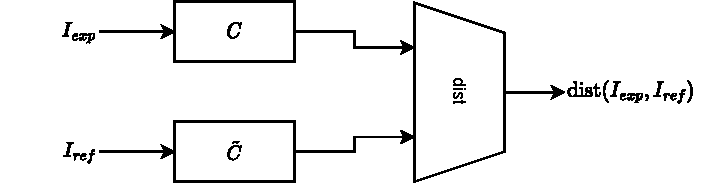
\includegraphics[height=3cm]{implementation/dist_ctf}
         \caption{CTF to reference}
         \label{fig:4:wiener:ctf}
    \end{subfigure}\\
    \vspace{2em}
    \begin{subfigure}[b]{\textwidth}
         \centering
         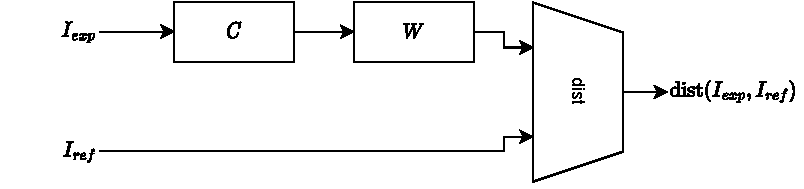
\includegraphics[height=3cm]{implementation/dist_wiener}
         \caption{Wiener correction}
         \label{fig:4:wiener:wiener}
    \end{subfigure}\\
    Where $C$ is the \gls{ctf}, $\tilde{C}$ is the \gls{ctf} estimation and $\tilde{C}^{-1}$ is the Wiener filter for correcting the estimated \gls{ctf}.
    \caption{CTF correction approaches}
    \label{fig:4:wiener}
\end{figure}

Among other applications, the Wiener filter can be used to deduce the inverse filter for a \gls{lti} system, as is the case of the \gls{ctf} model. This process is also known as the Wiener deconvolution. The definition of the Wiener inverse filter is displayed at \eqref{eq:4:wiener}, which also expresses it in function of the \gls{ssnr}. Note that in absence of noise (infinite \gls{ssnr}), the filter tends to behave as the inverse filter\cite{wetzstein2018}. The term $N(f)/S(f)$ is usually refereed as the Wiener constant, which prevents overamplification when the direct filter's gain is low. Note that the $S(f)$ terms refers to the signal \gls{psd} before the direct filter, whilst the $N(f)$ term refers to the noise \gls{psd} after the filter. This signals are represented in the block diagram of Figure \ref{fig:4:wiener_block}.

\begin{equation}\label{eq:4:wiener}
\begin{split}
    \hat{H}^{-1}(f) = 
    \frac{H^*(f) \cdot S(f)}{\left\vert H(f) \right\vert^2 \cdot S(f) + N'(f)} = 
    \frac{H^*(f)}{\left\vert H(f) \right\vert^2 + \frac{N'(f)}{S(f)}} = \\
    \frac{1}{H(f)} \cdot \frac{\frac{S(f)}{N'(f)} \cdot \left\vert H(f) \right\vert^2}{\frac{S(f)}{N'(f)} \cdot \left\vert H(f) \right\vert^2 + 1}
\end{split}
\end{equation}

\begin{figure}[htbp]
    \centering
    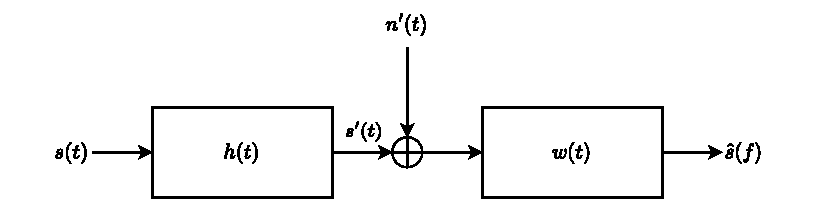
\includegraphics[width=.75\textwidth]{implementation/wiener}
    \caption{Wiener deconvolution block diagram}
    \label{fig:4:wiener_block}
\end{figure}

The Wiener filter was already implemented in Xmipp\cite{sorzano2004} as \texttt{xmipp\_ctf\_correct\_wiener2d} program, so the existing implementation was re-used for this algorithm. This program assumes a constant \gls{ssnr} profile across all frequencies. This constant \gls{ssnr} value is derived from the Filter's mean energy. It has been empirically proven that using a $10\si{\percent}$ of the filter's energy leads to good results\cite{grigorieff2017}.

The main drawback of this approach is that the Wiener filter is not able to correct frequencies where the direct filter has a zero. As shown in \eqref{eq:4:wiener_zero}, the Wiener inverse filter has also a zero for those frequencies, hence, those frequencies will not be at its output. In addition, the Figure \ref{fig:2:ctf} points out that the \gls{ctf} has periodic zero crossings, which will be subjected to this phenomenon.

\begin{equation}\label{eq:4:wiener_zero}
    \lim_{\left\vert H(f) \right\vert \rightarrow 0} \hat{H}^{-1}(f) = 0
\end{equation} 

As a consequence, some spatial frequencies are not present in the experimental image to be compared, but they are potentially present in the artificially generated image. This will induce a systematic error when comparing images. However, according to the experiments detailed later, we have not observed any significant influence of this effect. 

\subsection{Search vector description}
Image comparisons can be formulated as vector comparisons. From now on we will consider image comparisons as abstract vector comparisons. The easiest way to turn an image into a vector is by flattening all its pixels into a single dimension. For instance, all the rows of a given image could be concatenated to form a vector. In other words, the search vector will have as many dimensions as the number of pixels on an image. A typical image size of $160\times160$ would require a vector of size $25600$. This means that vectors will have a very high dimensionality, with the associated computational and storage cost.

It has been empirically proven that most of the alignment information is below a resolution of $6-8 \si{\angstrom}$\cite{scheres2021}. This means that a downsampled version of the image could be used. Provided that the $160\times160$ image was captured with a pixel size of $2 \si{\angstrom}$, it could be downsampled with a factor of $2$, which would lead to a vector size of $6400$. 

What is more, because of the orthonormality of the \gls{dft}, the comparisons can be performed in Fourier space. This allows to extract coefficients from a disc with the radius of the resolution limit. This disc involves slightly less coefficients due to the fact that it is inscribed inside the downsampled Fourier space. The DC component of the image can also be omitted, as it does not provide any information for alignment. In the example shown in the Figure \ref{fig:4:downsampling}, the Fourier disc has $2512$ complex coefficients. For our purposes, complex coefficients can be flattened to a vector twice as large. For the previous example, this leads to a vector of $5024$ dimensions, slightly less than the downsampled version of the image.

\begin{figure}[htbp]
    \centering
    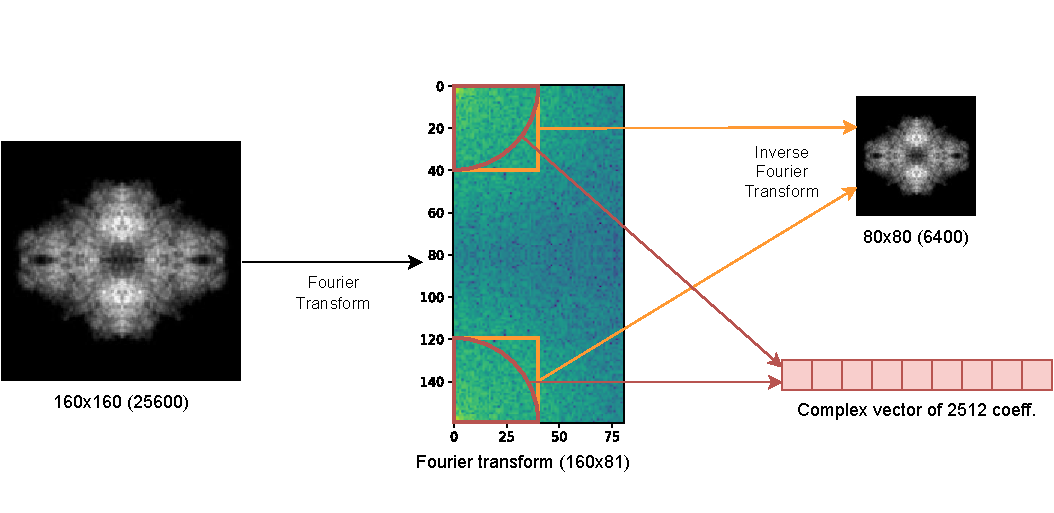
\includegraphics[width=\textwidth]{implementation/downsampling}
    \caption{Comparison of downsampling and coefficient extraction}
    \label{fig:4:downsampling}
\end{figure}

We have observed slightly more accurate results when using the \gls{dct} instead of the \gls{dft} for a given disc size. However, the cost of computing the \gls{dct} is also greater.

As a consequence, we will select a low frequency disc in Fourier space to transform all images into a search vector. As shown in the previous example, the images can be reduced by a factor of $5$ at little accuracy cost. In the results chapter, we will discuss the accuracy loss that can be attributed to discarding high frequency information.

\subsection{Reference gallery generation}
The reference gallery generation was formally described in Chapter \ref{chap:state_of_the_art}. The aim of this section is to describe the practical implementation used for this algorithm. This implementation groups alignment parameters in such a way that intermediary images can be stored and used repeteadly, avoiding redundant computations.

The first group is formed by the tilt and rot Euler angles which describe the projection direction. Using the \texttt{xmipp\_angular\_project\_library}\cite{sorzano2004} program, a set of equally spaced projections of the reference volume is generated. This set of images has all the considered variations of the tilt and rot Euler angles.

Then, each of these projected images is rotated in its own plane by a set of equally distributed angles, adding the third and last Euler angle variation, psi. At this point, the images are transformed to Fourier space, so that the low frequency disc can be extracted as described earlier. In theory, this last operation could be done before applying the in-plane rotations to the images, which would imply far less repetitions of this operation. However, this is not feasible in practice because interpolating Fourier coefficients tends produce incorrect results.

Finally, a set of shift filters is applied to the extracted Fourier coefficients. This operation can be performed in Fourier space because a shift filter is a \gls{lti} system, which is applied as a point operation to the Fourier coefficients. Hence, it can be only applied to the coefficients extracted from the disc. The \gls{dft} of the shift filter is defined as \eqref{eq:4:shift} where $\bm{\Omega}$ is the frequency vector and $\bm{\Delta}$ is the shift vector in pixels.

\begin{equation}\label{eq:4:shift}
    H(\bm{\Omega}) = e^{-j\bm{\Omega} \cdot \bm{\Delta}}
\end{equation}

The whole process has been illustrated in Figure \ref{fig:4:gallery}. At the end, a vast amount of vectors is generated, representing all possible combinations of projection directions and in-plane transforms. Each experimental image will be searched across this collection of vectors to find a best match.

\begin{figure}[htbp]
    \centering
    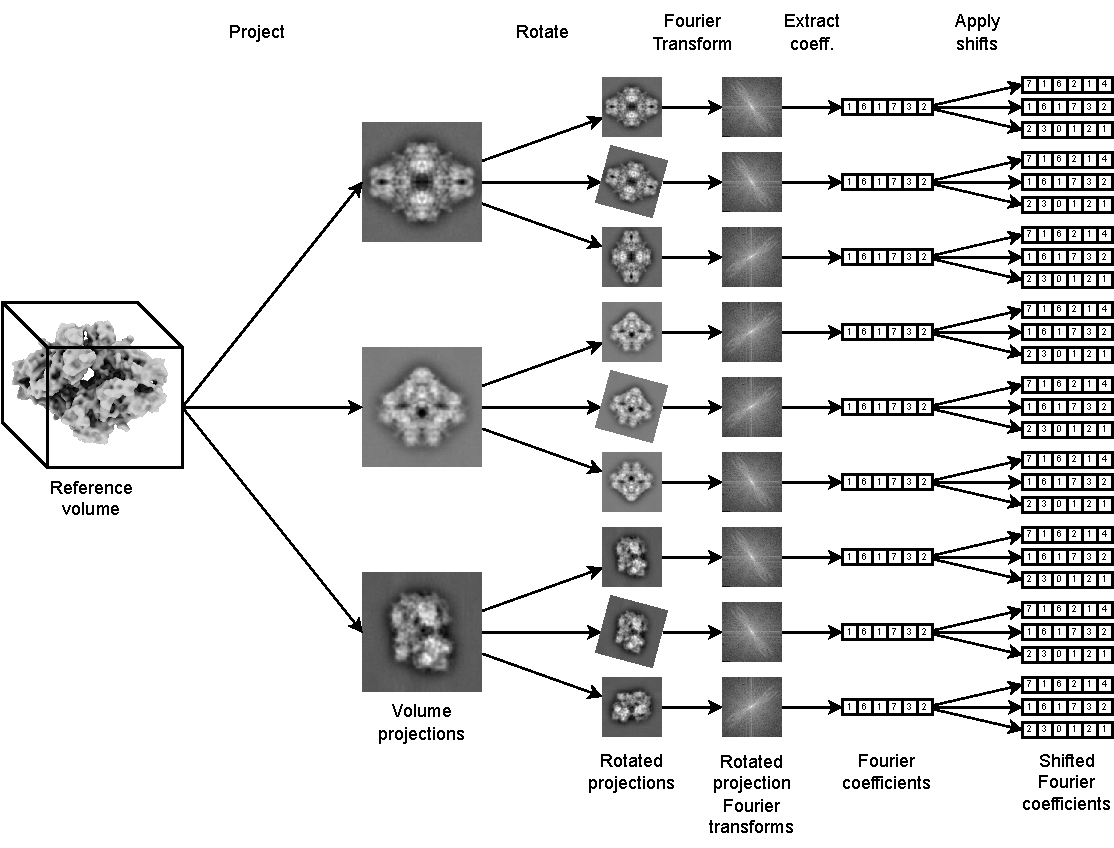
\includegraphics[width=\textwidth]{implementation/gallery}
    \caption{Gallery generation}
    \label{fig:4:gallery}
\end{figure}

\subsection{Vector search techniques}
At this point, our goal is to find the most similar vector across the previously generated dataset for each experimental image. In the context of \gls{ml}, this problem is known as \gls{knn}. One of the main strengths of this algorithm is the usage of state-of-the-art vector search techniques. In particular, we have used the FAISS library\cite{johnson2019}, developed by Facebook Research. This library is known to be one of the fastest vector search utilities. Moreover, it supports input from the Torch library, which eases interfacing with the rest of the program.

FAISS allows to build very complex vector databases with a modular structure. Depending on this structure, the expected size and dimensions, it may be suitable to fit entirely in \gls{cpu} memory or even \gls{gpu} memory. This is specially useful for modules designed to take advantage of \gls{gpu} accelerators. Moreover, this is also beneficial if data is already at the \gls{gpu}, as it avoids making expensive copies between \gls{gpu} and \gls{cpu} memory.

We have deduced that the former gallery generation approach can easily reach a size of many million of images. Provided that each image is represented by a couple of thousands coefficients, it can be easily inferred that storing all these coefficients in a raw array would require many Gigabytes. This may fit in high-end server \gls{cpu} memory, but it is unthinkable to store this amount of information on a \gls{gpu}.

Therefore, we have chosen to use FAISS's vector quatization and compression techniques. These methods are designed to compress vectors into a handful of bytes, enabling to store huge datasets in \gls{gpu} memory. However, these compression techniques come at an accuracy cost. This accuracy loss is highly dependant on the nature of the data itself, as highly correlated data will tend to compress well, whilst independent variables will produce a significant degradation of quality. We will discuss the influence of these compression algorithms with \gls{cryoem} data in Chapter \ref{chap:results}.

We have opted to use the database architecture recommended by FAISS guidelines\cite{johnson2019} that best represents the magnitudes of our data estimates. This architecture uses the \gls{pq} vector compression technique to achieve aforementioned compression ratios. On top of it, it uses a \gls{ivf} data structure to accelerate searches. We have also selected these techniques because they have been implemented for \glspl{gpu}, so that the whole search process can be run in these accelerators. A brief description of these techniques is provided hereafter.

\subsubsection{Product Quantisation}
\Glsfirst{pq} is a vector compression technique suitable for performing efficient \gls{knn} searches. Unlike other vector compression techniques, it has been designed to work well with large vectors\cite{chang2022a}\cite{jegou2011}.

This algorithm splits each vector into fixed sized chunks, which will be individually treated. The last chunk may be padded with zeros if necessary. A example of this partition is shown in Figure \ref{fig:4:pq_division}.

\begin{figure}[htbp]
    \centering
    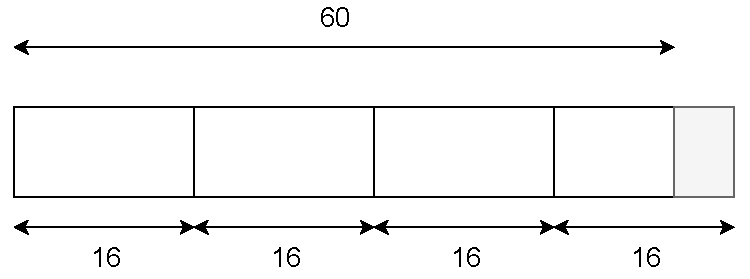
\includegraphics[width=.6\textwidth]{implementation/pq/vector}
    \caption{Example of vector partitioning for the PQ compression algorithm}
    \label{fig:4:pq_division}
\end{figure}

At the beginning, the \gls{pq} encoder needs to be trained with a representative subset of the dataset. In this training process, a k-means is executed for each chunk of the vector, producing $k$ centroids. This process is illustrated in Figure \ref{fig:4:pq_kmeans}. K-means is a unsupervised clustering algorithm that groups points in such a way that the distance to the centroid of their corresponding class is minimized\cite{sontag2012}. K-means requires the training set to be much larger than $k$ in order to be effective.

\begin{figure}[htbp]
    \centering
    \includegraphics[width=.7\textwidth]{implementation/pq/kmeans}
    \caption{K-means usage for PQ vector compression}
    \label{fig:4:pq_kmeans}
\end{figure}

At this point, the \gls{pq} encoder can be used to encode new vectors. The encoding consists in matching the closest centroid for each chunk of the vector. Hence, the vector can be encoded with a set centroid identifiers. This sequence of identifiers is known as \gls{pq}-code\cite{chang2022a}. Provided that $k$ centroids have been computed for each chunk, $\lceil \log_2 k \rceil$ bits are required to index each chunk. In total, $N \cdot \lceil \log_2 k \rceil$ bits will be necessary to store a vector, $N$ being the number of chunks\cite{briggs2022}. At most $k^N$ unique vectors can be represented with this technique. Beyond this number, code collisions are guaranteed to occur.

\begin{figure}[htbp]
    \centering
    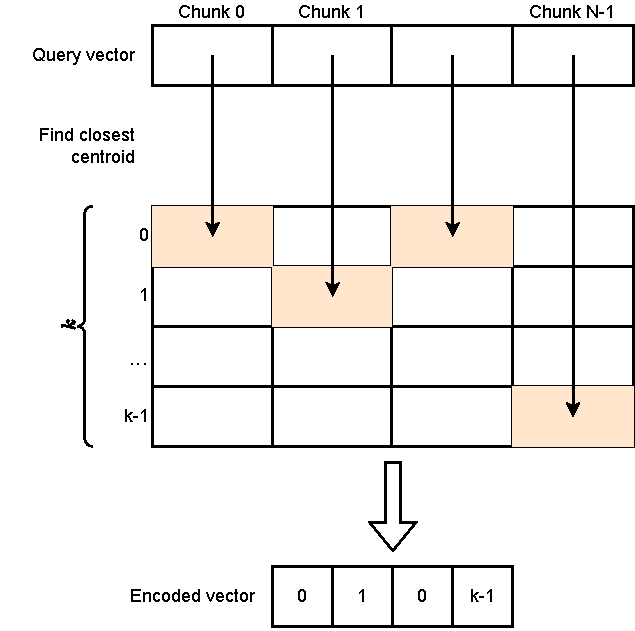
\includegraphics[width=.7\textwidth]{implementation/pq/encoding}
    \caption{Example of PQ encoding}
    \label{fig:4:pq_encoding}
\end{figure}

Decoding \gls{pq} codes is not necessary for our purpose, but it can be achieved. This process would involve following the inverse path of the Figure \ref{fig:4:pq_encoding}. This is, centroids would be indexed according to the encoded \gls{pq}-codes and then concatenated to ensemble a vector.

This technique also allows to efficiently compute distances between a given pair of encoded vectors. To do so, all the pairwise squared euclidean distances between centroids are precomputed and stored in memory. Then, it is a matter of indexing and accumulating this precomputed distance for each chunk. Figure \ref{fig:4:pq_distance} illustrates this distance computation process for the squared Euclidean distance. However, this idea can be extended for many other distance metrics. Note that the figure illustrates pairwise distances with a matrix. In practice, matrices are not used to store pairwise distances, as they are inefficient due to the symmetry of the distance functions ($\text{dist}(\bm{A}, \bm{B}) = \text{dist}(\bm{B}, \bm{A})$) and trivial cases ($\text{dist}(\bm{A}, \bm{A}) = 0$).  

\begin{figure}[htbp]
    \centering
    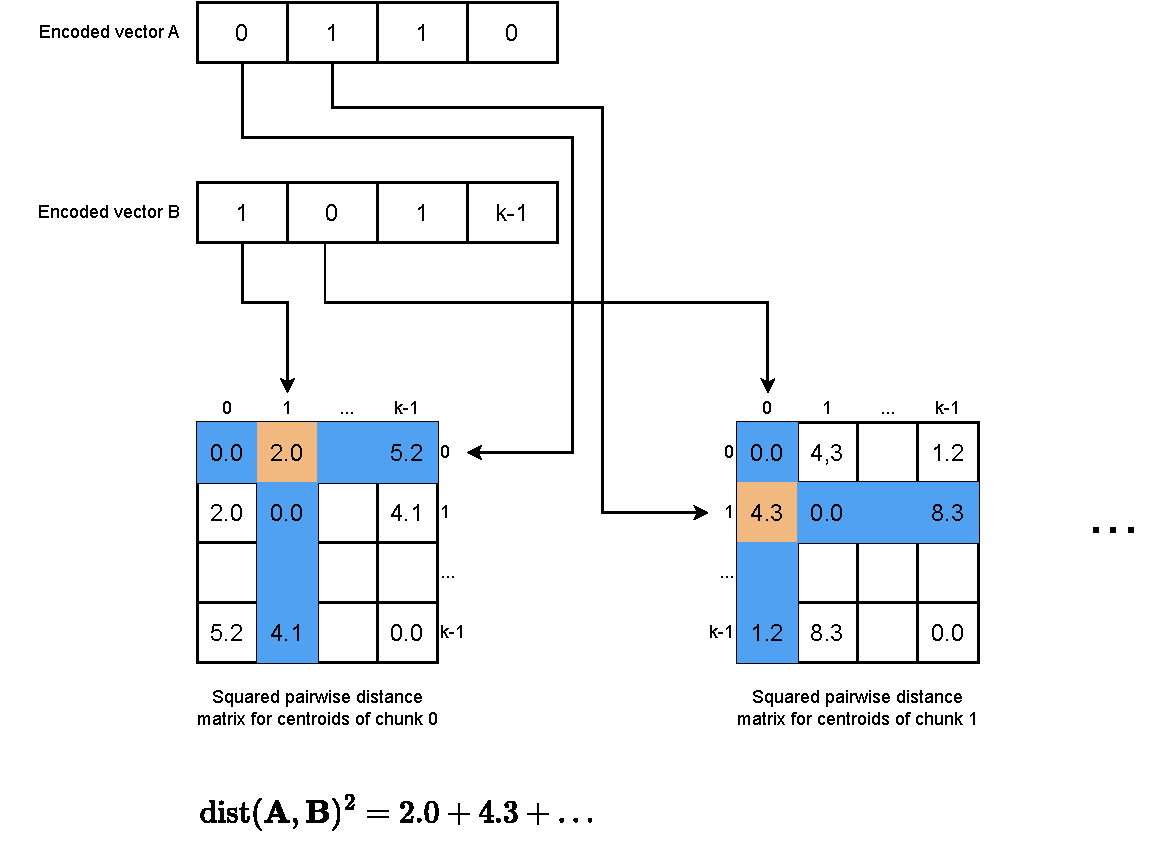
\includegraphics[width=\textwidth]{implementation/pq/distance}
    \caption{Example of PQ distance calculation}
    \label{fig:4:pq_distance}
\end{figure}

Having a fast distance estimate accelerates \gls{knn} vector searches, as these involve comparing a given vector against all the vectors in the dataset. Nevertheless, \gls{pq} comes with its own drawbacks. As its name suggests, it is a quantisation procedure, hence, there will be some accuracy loss. This accuracy loss is determined by the dispersion of the data. If the data is structured in a few compact clusters, K-means will be able to identify them and the quantisation error will be minimal. Contrary to this, if the data is random, the centroids may not be representative and a lot of quantisation error will be introduced.

The quantisation loss can be minimised applying a linear transform to the vectors before quantizing them. This linear transform is represented with a rotation matrix, which will rotate vectors in such a way that the quantisation error is minimised. Due to the fact that rotation matrices are orthonormal, distances are preserved after this rotation\cite{ge2013}. 

\subsubsection{Inverted File}
\Gls{pq} provides a compact way to store vectors and reduce distance computation time. However, it is not effective enough when searching across millions of vectors\cite{chang2022b}. Therefore, it is usually complemented with \glsfirst{ivf} to significantly reduce search times.

\Gls{ivf} works by limiting the search scope for a particular query vector. To do so, once again K-means is used. This time, K-means is used to partition the entire vector space (instead of a small set of axes). Once again, this partition is done in the training process, so a large enough represetentive subset of the data needs to be provided. This process will provide a coarse quatization of the vector space in discrete cells, which can be seen as Voronoi cells\cite{chang2022b}. These cells can be used to limit the extent of the searches.

Once the database has been trained, vectors are grouped according to their closest centroid. Then \gls{pq} will be used to encode the residual vector from the centroid. A example of this partitioning is provided in Figure \ref{fig:4:ivf_kmeans}. Therefore, a vector will be encoded as the index of its coarse centroid and the \gls{pq}-code assotiated to the residual vector\cite{chang2022b}.

\begin{figure}[htbp]
    \centering
    \includegraphics[width=.8\textwidth]{implementation/ivf/kmeans}
    \caption{K-means centroid and residual vector example for IVF searches}
    \label{fig:4:ivf_kmeans}
\end{figure}

When a search needs to be carried out, the query vector will also be assigned to the closest centroid. Then, the residual vector will be searched across all the residual vectors belonging to that group. However, this may pose a problem. If the query vector falls near the cell frontier, it is possible that the closest vector may be in the neighbouring cell. This case is exemplified with the $B$ point in Figure \ref{fig:4:ivf_search}, which gets assigned to the green region while its closest point is on the blue region. To solve this issue, each query vector is also searched across multiple neighbouring cells\cite{chang2022b}. 

\begin{figure}[htbp]
    \centering
    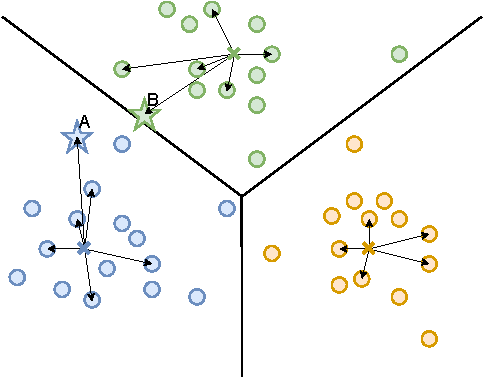
\includegraphics[width=.8\textwidth]{implementation/ivf/search}
    \caption{IVF search example}
    \label{fig:4:ivf_search}
\end{figure}

\subsubsection{Distance metric}
Until this point we have used the distance term without defining a concrete distance function. This was to preserve generality, as several distance functions were implemented. The aforementioned \gls{ivf}-\gls{pq} encoding only allows for Euclidean distance minimisation and dot product maximisation. In fact, these metrics are related to one another:

\begin{equation}\label{eq:4:dot_l2}
    \left\lVert \bm{x} - \bm{y} \right\rVert^2 =
    \left\lVert \bm{x} \right\rVert^2 + \left\lVert \bm{y} \right\rVert^2 - \left\langle \bm{x},\bm{y} \right\rangle
\end{equation}

Nevertheless, these metrics can be used as a basis to define many other distance metrics. For instance, the cosine similarity can be defined in terms of the dot product by providing normalised vectors.

\begin{equation}\label{eq:4:cos}
    \cos \theta = \left\langle \frac{\bm{x}}{\lVert \bm{x} \rVert} , \frac{\bm{y}}{\lVert \bm{y} \rVert} \right\rangle
\end{equation}

Similarly, the Pearson correlation can be calculated by subtracting the mean before calculating the cosine distance:

\begin{equation}\label{eq:4:pearson}
    \rho = \left\langle \frac{\bm{x} - \bm{\bar{x}}}{\lVert \bm{x} - \bm{\bar{x}} \rVert} , \frac{\bm{y - \bm{\bar{y}}}}{\lVert \bm{y} - \bm{\bar{y}} \rVert} \right\rangle
\end{equation}

Lastly, the weighted Euclidean distance can be calculated by scaling vector coefficients before computing the Euclidean distance:

\begin{equation}\label{eq:4:l2_w}
    \left\lVert \bm{x} - \bm{y} \right\rVert^2_{\bm{w}} = \left\lVert W(\bm{x} - \bm{y}) \right\rVert^2
\end{equation}

where 

\begin{equation}
    W = \text{diag}(\bm{w})
\end{equation}

Note that the previous definitions have been stated for real numbers. However, our vectors have been ensembled from complex vectors by interleaving their real and imaginary part:

\begin{equation}
    \bm{x} = 
    \begin{bmatrix}
        \Re(\hat{x}_1) & \Im(\hat{x}_1) & \Re(\hat{x}_2) & \Im(\hat{x}_2) & \dots  
    \end{bmatrix}
\end{equation}

This vector construct preserves the Euclidean norm from its original complex form and $+/-$ properties. Therefore, the euclidean distance remains valid.

\begin{equation}
    \left\lVert \bm{x} \right\rVert^2 = \bm{x}^T\bm{x} = \Re(\hat{x}_1)^2 + \Im(\hat{x}_1)^2 + \dots
\end{equation}
\begin{equation}
\begin{split}
    \left\lVert \bm{\hat{x}} \right\rVert^2 = \bm{\hat{x}}^H\bm{\hat{x}} =\\
    \Re(\hat{x}_1) \cdot \Re(\hat{x}_1) + \Im(\hat{x}_1) \cdot \Im(\hat{x}_1) +\\
    \cancel{j\Im(\hat{x}_1) \cdot \Re(\hat{x}_1)} - \cancel{j\Im(\hat{x}_1) \cdot \Im(\hat{x}_1)} + \dots =\\ \Re(\hat{x}_1)^2 + \Im(\hat{x}_1)^2 + \dots
\end{split}
\end{equation}

However, in general, the dot product is not preserved from one form to the other because it discards the imaginary part of the result:

\begin{align}
    \bm{x}^T\bm{y} &= \Re(\hat{x}_1) \cdot \Re(\hat{y}_1) + \Im(\hat{x}_1) \cdot \Im(\hat{y}_1) + \dots\\
    \bm{\hat{x}}^H\bm{\hat{y}} &= \Re(\hat{x}_1) \cdot \Re(\hat{y}_1) + \Im(\hat{x}_1) \cdot \Im(\hat{y}_1) + j \Re(\hat{x}_1) \cdot \Im(\hat{y}_1) + j\Im(\hat{x}_1) \cdot \Re(\hat{y}_1) + \dots
\end{align}

In spite of this, our particular case involves Fourier coefficients, which have symmetry. When considering symmetric pairs of coefficients, the imaginary part of the dot product cancels out. Hence, for this case, the dot product is preserved.

\begin{equation}
\begin{split}
    \bm{\hat{x}}^H\bm{\hat{y}} + (\bm{\hat{x}}^*)^H(\bm{\hat{y}}^*) =\\
    \Re(\hat{x}_1) \cdot \Re(\hat{y}_1) + \Im(\hat{x}_1) \cdot \Im(\hat{y}_1) + \cancel{j \Re(\hat{x}_1) \cdot \Im(\hat{y}_1)} + \cancel{j\Im(\hat{x}_1) \cdot \Re(\hat{y}_1)} +\\ 
    \Re(\hat{x}_1) \cdot \Re(\hat{y}_1) + \Im(\hat{x}_1) \cdot \Im(\hat{y}_1) - \cancel{j \Re(\hat{x}_1) \cdot \Im(\hat{y}_1)} - \cancel{j\Im(\hat{x}_1) \cdot \Re(\hat{y}_1)} + \dots =\\ 
    2 \cdot (\Re(\hat{x}_1) \cdot \Re(\hat{y}_1) + \Im(\hat{x}_1) \cdot \Im(\hat{y}_1) + \dots)
\end{split}
\end{equation}

Considering these two facts, the flattened representation of the complex vector leads to numerically identical (and more efficient) results when computing distances and similarities.

\end{document}